\chapter{Concept and Design}
\label{cha:conceptanddesign}

We need to describe here what do we want to achieve, what do we mean by modelling and visualizing macroscopic movements etc - thus general architecture that we have 3 components, Stop Detection from telekom data based on movements and updates of "areas" in your mobile phone, Clustering of Stops to find most popular "stops" in the city, Graph Generation to find where do the people move and in what amount

\section{Stop Detection}

Analyzing different approaches for stop detection based on localization data (ref. \autoref{cha:introduction_appr_stopdet}), we decided to base our solution on standard human behavior regarding mobility within the cities (ref. \autoref{cha:introduction_hummob}) and reusing the concept of Mobility Index (ref. \autoref{cha:introduction_mob_index_sect})).
\\\\
Stop detection is divided into two phases:
\begin{description}
	\item[Identifying stop candidates] according to stop detection algorithm
	\item[Reconciliation of stop candidates] taking into account mobility indexes of points. 
\end{description}

\subsection{Identifying stop candidates}

Stop algorithm, shown on \autoref{fig:cd_algorithm}, is considering 3 parameters - MinWalkSpeed, MinTransportSpeed, ThresholdDistance. 
\\\\
So called ThresholdDistance is distance mentioned in \autoref{cha:introduction_dataanaly} (which in case of Berlin been in range 800-1500m) as distances between points, where there is significant "jump" in frequency of occurences, which might mean that at these intervals, continuous points been gathered, and distances over that values might be discontinuous. Furthermore, these distances are relatively small compared to other observed distances, allowing more accurate decision process. We assume, that at these distances, no significant "interuption" in gatharing the points has been introduced in the form of buildings, metro or other factors.
\\\\
Thus, for these higher accuracy points one could assume, that if mobile device have been moving within the minimum walking speed MinWalkSpeed (ref. \autoref{cha:introduction_hummob}), this point is identified as stop candidate. 
\\\\
Thus, for lower accuracy points one could assume, that if mobile device have been moving within the minimum transport speed MinTransportSpeed (ref. \autoref{cha:introduction_hummob}), this point is as well identified as stop candidate. In this example, it could mean, that over longer distance, one could move with transportation with significant speed, stop for longer period and then use fast transportation again, resulting in higher then minimum walking speed, but with speed which is in average lower then other psychological value as minimum transport speed or maximum walking speed.
\begin{figure}[!ht]
	\centering
	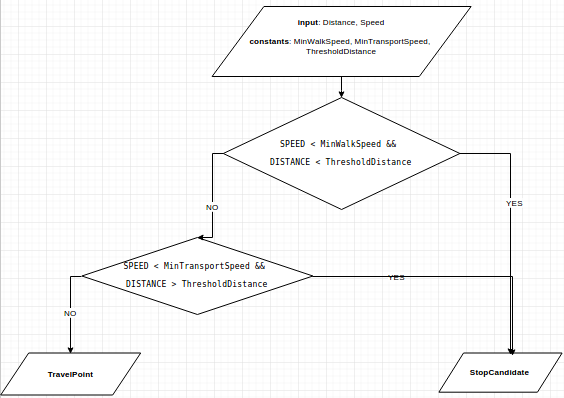
\includegraphics[width=0.8\textwidth]{images/stop_algorithm_1.png}\\
	\caption{First phase of stop detection algorithm  }
	\label{fig:cd_algorithm}
\end{figure}

\subsection{Mobility Index Analysis}

\autoref{fig:reco_general} shows that there are many scenarios in which stop candidate has been detected, taking into account movement speed between points, distance and mobility index. From the statistics about collection of points per user - \autoref{cha:introduction_dataanaly}) - the following movement profiles can be derived:
\\
\begin{description}
	\item[Standard daily movements with few relocations across the city] - In average mobile devices collected 17 points. The profile of this person could be matching e.g. - going to work in the morning, going for lunch and back, going to the shop/entertainment after work and home. This could result in points collected during transportation to those places (5-40). 
	\item[Relocations over small distances] - harmonic mean has been 4 points, which could mean that person during that day was indeed moving, but frequently requiring "area updates", thus distance covered daily was small. 
	\item[Many relocations over larger distances] - number of points collected in range above 60, might mean that user is moving a lot during the day (e.g. delivery, professional driver) or moves over long distance to another city. 
\end{description}
\begin{figure}[!ht]
	\centering
	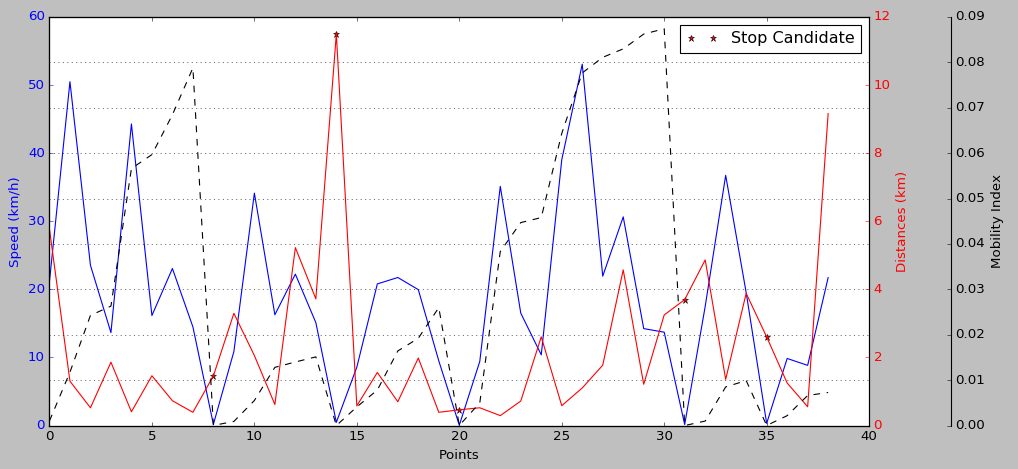
\includegraphics[width=0.8\textwidth]{images/reco_general.png}\\
	\caption{Result of identifying stop candidates for single user with their corresponding mobile index, distance and speed between the detected and previous point }
	\label{fig:reco_general}
\end{figure}
In the example for a single user over 24h shown on \autoref{fig:reco_general}, stop detection algorithm identified 5 stops. The dashed line represents the mobility index which was considering past 60 minutes from each of the points, representing how movable was that person in the last 60 minutes till that point. Analyzing mobility index in the above example (ref. \autoref{cha:introduction_mob_index_sect}), we identify "rising mobility periods" as periods of mobility/transportation, while rapid drop, as very low mobility/stay indicator.Worth notifying is that mobility index in that example very accurately correlates with the identified stop candidates. 
\begin{figure}[!ht]
	\centering
	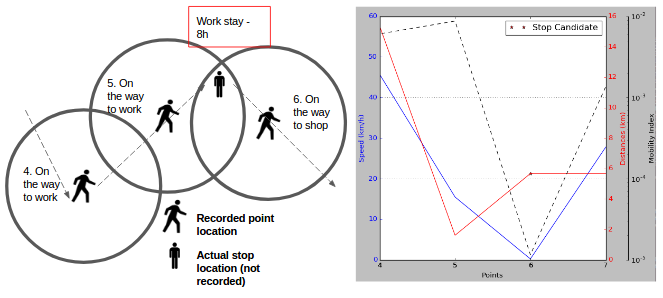
\includegraphics[width=0.9\textwidth]{images/reco_example_1.png}\\
	\caption{ Correlation of the real life example (left) to the graph of distance, speed and mobility index between consequtive points (right) }
	\label{fig:reco_ex_1}
\end{figure}
\\
Due to the method of obtaining the data - \autoref{fig:reco_ex_1} - one cannot precisely identify the location of the stop, it can be closer to Point 5, Point 6 or somewhere in the middle the two. Furthermore, statistically, most stops identified have  mobility index below certain threshold \textbf{(10e-3)} - which can be taken as a point of reference for other considerations - meaning that user continued movement, but with low speed.
\FloatBarrier

\subsection{Reconciliation of stop candidates}

\begin{figure}[!ht]
 	\centering
 	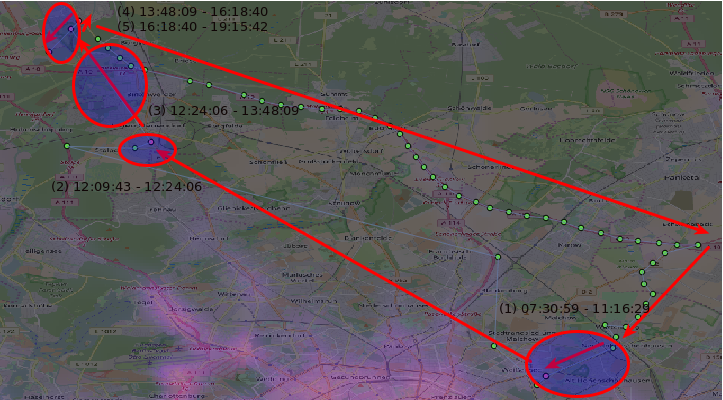
\includegraphics[width=0.6\textwidth]{images/reco_example_2b.png}
 	\caption{ Movement example for one user in the period of 24h, with recorded locations due to the movement and annotated timestamps for detected stop candidates }
 	\label{fig:reco_ex_2b}
\end{figure}
\begin{figure}[!ht]
 	\centering
 	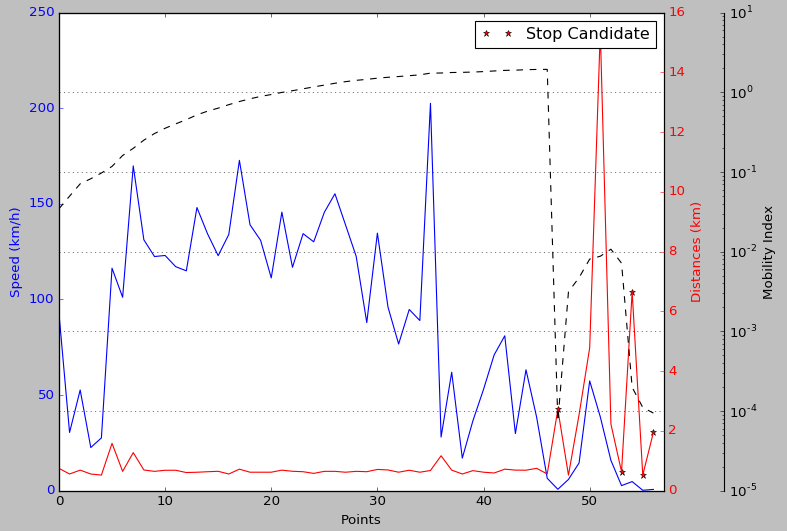
\includegraphics[width=0.6\textwidth]{images/reco_example_2a.png}
 	\caption{ Visualization of distances, speed and mobility indexes for example from \autoref{fig:reco_ex_2b} with identified stop candidates }
	\label{fig:reco_ex_2a}
\end{figure} 
Analyzing traces from \autoref{fig:reco_ex_2b} and \autoref{fig:reco_ex_2a}, we identify that user has been moving from Point 0 to Point 47, in the time period 06:59 - 07:30. In between Point 47 and Point 48, the stop candidate has been identified. We notice, that from Points 0-47, measurement has been continuously gathered over a distance. This could mean, that user stopped somewhere around Point 47, stayed there some time, and when he left that location, after around 3 km from that point, at 11:16 user has been recorded in location Point 48, starting his journey to Point 54. Thus, Stop Candidate at Point 48 is meaning in that case Stop might be close to Point 47 on that way (previous to stop candidate). 
\\\\
At Point 54, we recorded Stop Candidate, however, considering that its mobility index being high (above 10e-3, also validated by small distance and walking speed covered between 12:09-12:24) and next mobility index being low, we can assume that this Stop Candidate is not a stop and have to be ignored, it is most likely approaching to the stop location. 
\\\\
In between Points 54-55, we record another Stop Candidate, in period from 12:24-13:48 and over significant distance. Recorded mobility index is low, and because it is over long distance, we assume that Stop is close to Point 54 on the way to Point 55. 
\\\\
Due to the small distance covered in between Points 55-56 and Points 56-57, we expect that the Stop Points in that cases are somewhere in between or around these Points. 
\begin{figure}[!ht]
	\centering
	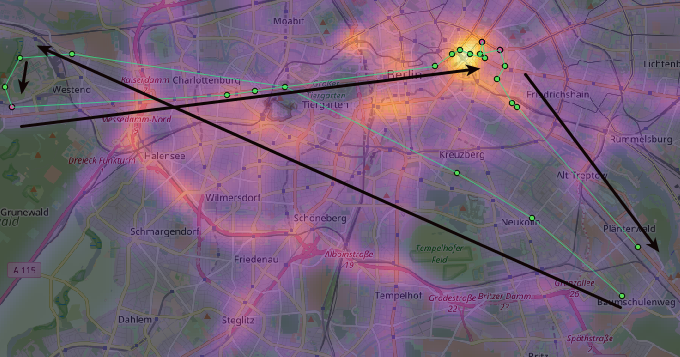
\includegraphics[width=0.6\textwidth]{images/reco_example_5a.png}
	\caption{ Visualization of distances, speed and mobility indexes for example from \autoref{fig:reco_ex_5b} with identified stop candidates }
	\label{fig:reco_ex_5a}
\end{figure} 
\begin{figure}[!ht]
	\centering
	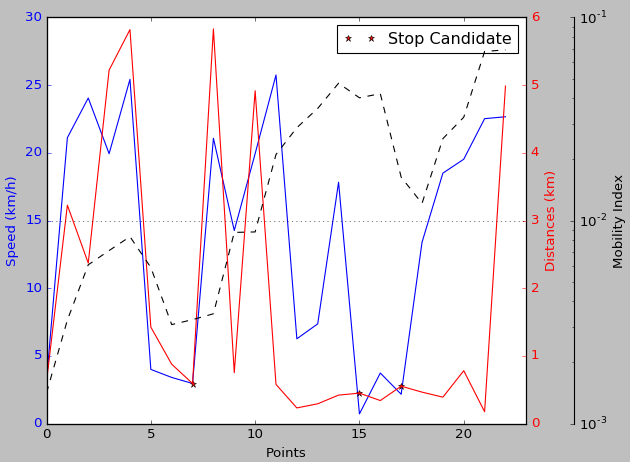
\includegraphics[width=0.6\textwidth]{images/reco_example_5b.png}
	\caption{ Movement example for one user in the period of 24h, with recorded locations due to the movement and annotated timestamps for detected stop candidates }
	\label{fig:reco_ex_5b}
\end{figure}
\\
Analyzing traces from \autoref{fig:reco_ex_5b} and \autoref{fig:reco_ex_5a} we identify example in which person is constantly moving between 8:28-12:04, and having 3 short stops in range 15-40 minutes, in Points 7, 15, 17. Mobility index in both examples is above the mobility index threshold, however, in the next point that person is again moving (above mobility index threshold), which might identify short stay at that location. 
\\\\
Further examples, showing the above mentioned events can be found in \autoref{appendix:add_example_1}, \autoref{appendix:add_example_2}
\\\\
TODO: Now should decide what should be algorithm based on above mentioned values, most probably for:
\\-> mobility index higher then the threshold, and next point mobility index being lower then the threshold, there is no stop, but slow movement to possible stop location. 
\\-> mobility index higher then the threshold, and next point mobility index being also higher then the threshold might mean that there is short stop at the location
\\-> short distance covered, stop is either in both current and previous or in between
\\-> for long distance the stop is close to previous point

\section{Clustering of Stops}

\FloatBarrier
\section{City Movements Graph}

\FloatBarrier